\section{Aufbau und Durchführung}
\subsection{Aufbau}
\label{sec:Aufbau}

Bei diesem Versuch wird ein Röntgengerät, dargestellt in Abbildung \ref{abb:1}, verwendet.
\begin{figure}[H]
  \centering
  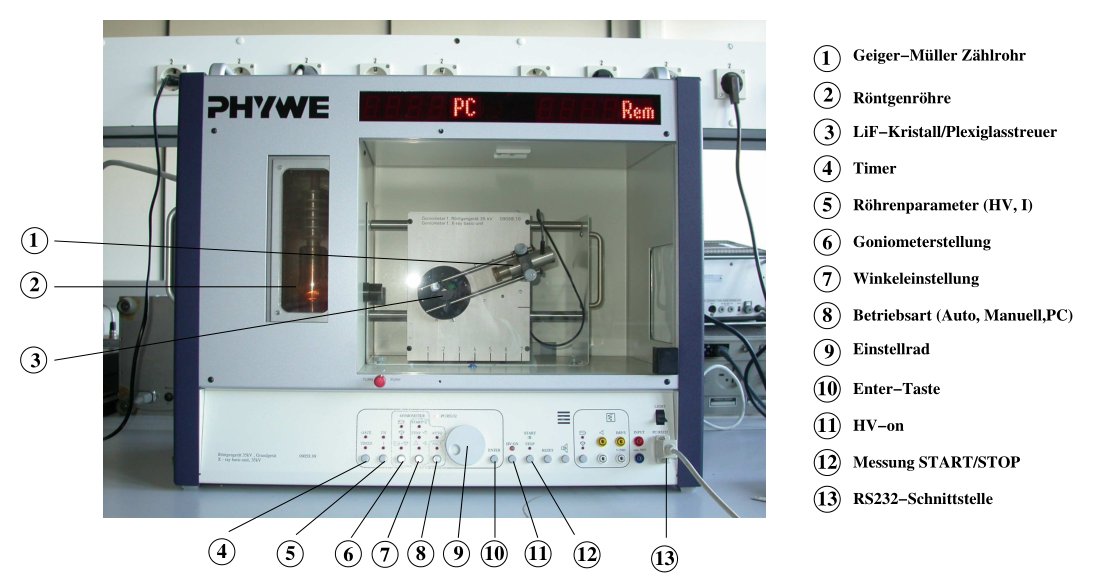
\includegraphics[height=8cm]{ressources/aufbau.png}
  \caption{Röntgengerät. \cite{skript}}
  \label{abb:1}
\end{figure}
Es besteht grundsätzlich aus einer Kupfer-Röntgen-Röhre, welche auf einen um sich selbst rotierbaren LiF-Kristall gerichtet ist.
Auf einer Kreisbahn um den Kristall kann wiederrum ein auf jenen gerichtetes Geiger-Müller-Zählerrohr bewegt werden.
Diese drei Hauptkomponenten sind mit einem Computer verbunden und über eine dafür entwickelte Software steuerbar.
Die Software nimmt die Zählrate in Abhängigkeit des Winkels des Kristalls auf.
Dabei können die Strom- und Spannungszufuhr der Röntgen-Röhre, sowie einzeln und simultan, beispielsweise im 2:1 Modus (das Zählrohr hat den doppelten Winkel des Kristalls), die Winkelläufe des Kristalls und Zählrohrs festgelegt und variiert werden.
Zusätzlich können der Winkelzuwachs und die Integrationszeit, also die Zeit in der jeder Winkel gehalten werden soll, eingestellt werden.\\
Für die Messung der Absorptionsspektren können vor das Geiger-Müller-Zählrohr Blenden mit verschiedenen Absorbern geschraubt werden.
Es ist zu beachten, dass Röntgengerät nur im geschlossenen Zustand laufen zu lassen.
